\documentclass[10pt,a4paper]{article}
\usepackage[margin=15mm,top=13mm,bottom=13mm]{geometry}
\usepackage[T1]{fontenc}
\usepackage{newtxtext,newtxmath}
\usepackage{amsmath,mathtools}
\usepackage{booktabs,tabularx,array}
\usepackage{tikz}
\usetikzlibrary{arrows.meta,positioning,calc}
\usepackage{microtype}
\usepackage{enumitem}
\usepackage{fancyhdr}
\usepackage{float}
\usepackage{titlesec}
\titleformat{\section}{\normalfont\fontsize{11}{12}\bfseries}{\thesection}{0.5em}{}
\titleformat{\subsection}{\normalfont\fontsize{10}{11}\bfseries}{\thesubsection}{0.5em}{}
\titlespacing*{\section}{0pt}{7pt}{3pt}
\titlespacing*{\subsection}{0pt}{5pt}{2pt}
\titleformat{\paragraph}[block]{\normalfont\fontsize{10}{11}\bfseries}{}{0pt}{}
\titlespacing*{\paragraph}{0pt}{5pt}{1pt}
\newcommand{\notation}[2]{\noindent\textbf{#1}\par\nopagebreak #2\par}
\usepackage{hyperref}
\hypersetup{hidelinks,hypertexnames=false}
\setlength{\parindent}{0pt}
\setlength{\parskip}{2.5pt}
\linespread{0.96}
\setlength{\abovedisplayskip}{4pt}
\setlength{\belowdisplayskip}{4pt}
\setlength{\abovedisplayshortskip}{3pt}
\setlength{\belowdisplayshortskip}{3pt}
\pagestyle{fancy}\fancyhf{}\fancyfoot[C]{\footnotesize\thepage}\renewcommand{\headrulewidth}{0pt}
\renewcommand{\arraystretch}{1.2}
\newcommand{\GI}{\mathcal G_{\mathrm I}}
\newcommand{\GR}{\mathcal G_{\mathrm R}}
\newcommand{\RI}{\mathcal R_{\mathrm{2D}}}
\newcommand{\RR}{\mathcal R_{\mathrm{3D}}}
\newcommand{\RRf}{\mathcal R_{\mathrm{3D}}^{\mathrm{front}}}
\newcommand{\Vf}{\mathcal V_{\mathrm{dyn}}}
\newcommand{\Def}{\mathcal D}
\newcommand{\uu}{\mathbf u}
\newcommand{\nn}{\mathbf n}
\newcommand{\cc}{\mathbf c}

\newcommand{\Om}{\Omega}
\newcommand{\smallcap}[1]{{\fontsize{8.5}{10.5}\selectfont #1}}
\tikzset{box/.style={draw=black!70,line width=.45pt,align=center,inner sep=4pt,minimum height=9mm,font=\footnotesize},
 flow/.style={-{Latex[length=2mm]},line width=.55pt},
 rev/.style={-{Latex[length=2mm]},line width=.5pt,densely dashed}}
\newcommand{\notepair}[4]{\par\noindent
\begin{minipage}[t]{0.485\textwidth}\small\notation{#1}{#2}\end{minipage}\hfill
\begin{minipage}[t]{0.485\textwidth}\small\notation{#3}{#4}\end{minipage}\par\vspace{1pt}}
\begin{document}
\begin{center}
{\Large\bfseries VIGOR-GS}\\[2pt]
{\large Virtual-View Interface-Guided Optical Reflection Gaussian Splatting}\\[2pt]
{\footnotesize Technical framework --- training and inference}
\end{center}
\vspace{-1mm}\hrule\vspace{2mm}

\section*{1. Model and available inputs}
The interface is a set of 2D Gaussian disks~\cite{huang2024}; reflected appearance uses 3D Gaussian ellipsoids~\cite{kerbl2023}. With $N_{\mathrm I}$ disks and $N_{\mathrm R}$ ellipsoids, the canonical fields are
\begin{equation*}
\GI^0=\{(\boldsymbol\mu_i,q_i,\mathbf s_i^{(2)},p_i,o_i,\mathbf a_i)\}_{i=1}^{N_{\mathrm I}},
\qquad
\GR^0=\{(\boldsymbol\mu_j,q_j,\mathbf s_j^{(3)},o_j,\mathbf a_j)\}_{j=1}^{N_{\mathrm R}}.
\end{equation*}
\notepair{Center $\boldsymbol\mu\in\mathbb R^3$}{Position of the primitive in world coordinates.}
{Orientation $q$}{Unit quaternion specifying its 3D rotation.}
\notepair{Disk scales $\mathbf s^{(2)}\in\mathbb R_{>0}^{2}$}{Two in-plane Gaussian widths; rotation sets the normal.}
{Ellipsoid scales $\mathbf s^{(3)}\in\mathbb R_{>0}^{3}$}{Three Gaussian widths along the rotated axes.}
\notepair{Occupancy $p_i\in[0,1]$}{Learned soft presence of interface disk $i$.}
{Opacity $o\in[0,1]$}{Learned opacity conditional on primitive presence.}
\notepair{Appearance $\mathbf a$}{Color coefficients, optionally view dependent.}
{Effective interface opacity $\widetilde o_i=p_i o_i$}{2DGS uses this product~\cite{vigor}; 3DGS uses $o_j$.}
The two fields have independent parameters. Following canonical-space deformation~\cite{yang2024}, deformation MLPs change their geometry over time; interface occupancy and opacity are time independent:
\begin{equation}
\GI(t)=\Def_{\phi_{\mathrm I}}(\GI^0,t),
\qquad
\GR(t)=\Def_{\phi_{\mathrm R}}(\GR^0,t). \tag{1}
\end{equation}
Training uses $I_t$, clean targets $I_t^{\mathrm{clean}}$, and real cameras $C_t$.
Instead of one plane, assume $K$ known, fixed glass patches:
\begin{equation*}
\mathcal P=\{\Pi_k=(\mathbf n_k,d_k,\mathcal S_k)\}_{k=1}^{K},\qquad
\mathbf n_k^\top\mathbf x+d_k=0,\quad\|\mathbf n_k\|_2=1.
\end{equation*}
$\mathcal S_k$ is the finite 3D extent of glass patch $k$, from known geometry or the Phase~I interface geometry. The patches occupy different locations in 3D and may have different normals. A primary camera ray meets at most one \emph{selected visible} patch (the nearest hit if projections overlap). There is no learned image-space plane mask. Both Gaussian fields remain shared; primitive occupancy is not a plane-assignment variable.

\section*{2. Training: two sequential phases}
\textbf{Reading the losses.} $\Om$ is the nonempty set of evaluated image pixels, and $|\Om|$ is its pixel count. $\|A-B\|_1$ adds the absolute differences within one pixel. $\sum_{\uu\in\Om}$ adds these pixel errors, and dividing by $|\Om|$ gives the error per pixel. Each nonnegative $\lambda$ sets a penalty's strength; zero disables it. Loss weights are chosen for this per-pixel normalization.
\begin{figure}[H]
\centering
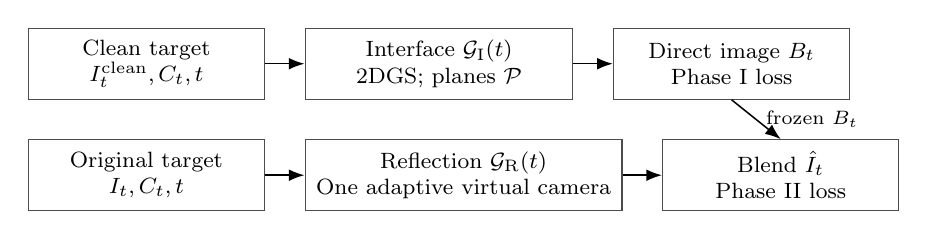
\begin{tikzpicture}[node distance=5mm]
\node[box,minimum width=30mm] (a) {Clean target\\$I_t^{\mathrm{clean}},C_t,t$};
\node[box,right=of a,minimum width=34mm] (b) {Interface $\GI(t)$\\2DGS; planes $\mathcal P$};
\node[box,right=of b,minimum width=30mm] (c) {Direct image $B_t$\\Phase I loss};
\node[box,below=5mm of a,minimum width=30mm] (d) {Original target\\$I_t,C_t,t$};
\node[box,right=of d,minimum width=34mm] (e) {Reflection $\GR(t)$\\One adaptive virtual camera};
\node[box,right=of e,minimum width=30mm] (f) {Blend $\hat I_t$\\Phase II loss};
\draw[flow] (a)--(b);\draw[flow] (b)--(c);
\draw[flow] (d)--(e);\draw[flow] (e)--(f);
\draw[flow] (c.south)--node[right,font=\scriptsize]{frozen $B_t$}(f.north);
\end{tikzpicture}
\caption{Forward training flow (framework design). Fit the interface first, then freeze it and fit the reflection field. One virtual-camera function rotates and repositions its view using the currently selected 3D glass plane.}
\end{figure}

\subsection*{Phase I: interface reconstruction}
Render the interface through the real camera using 2DGS~\cite{huang2024}:
\begin{equation}
B_t=\RI\bigl(\GI(t),C_t\bigr). \tag{2}
\end{equation}
\notepair{Interface field $\GI(t)$}{2D Gaussian disks deformed to timestamp $t$.}
{Real camera $C_t$}{Camera intrinsics and pose at timestamp $t$.}
\notepair{Rasterizer $\RI$}{The 2DGS renderer.}
{Direct image $B_t$}{Interface RGB render using effective opacities $p_i o_i$.}
Compare the render with the clean target:
\begin{equation}
\mathcal L_{\mathrm I}=\frac{1}{|\Om|}\sum_{\uu\in\Om}
\bigl\|B_t(\uu)-I_t^{\mathrm{clean}}(\uu)\bigr\|_1
+\lambda_{\mathrm s}\mathcal L_{\mathrm{surf}}. \tag{3}
\end{equation}
\notepair{Pixel $\uu$ and time $t$}{An image location and the time of the frame being rendered.}
{Clean target $I_t^{\mathrm{clean}}$}{The reflection-removed training image.}
\notepair{Image error in Eq.~(3)}{Absolute rendered-versus-clean error at each pixel, added over the image and divided by the pixel count.}
{Training goal}{Make the direct render look like the clean image.}
\notepair{Surface loss $\mathcal L_{\mathrm{surf}}$}{Surface-direction agreement, defined in Eq.~\eqref{eq:surf}.}
{Surface weight $\lambda_{\mathrm s}\geq0$}{Controls the strength of the geometry penalties.}
\subsection*{Surface loss: make the surface directions agree}
\textbf{Idea.} The disks describe a surface direction. The rendered depth also suggests a surface direction. Encourage these two descriptions to agree, following the normal-consistency idea in 2DGS~\cite{huang2024}:
\begin{equation}
\boxed{\mathcal L_{\mathrm{surf}}(t)=\frac{1}{|\Om_{\mathrm s}(t)|}
\sum_{\uu\in\Om_{\mathrm s}(t)}
\bigl\|N_t(\uu)-N_t^{\mathrm{depth}}(\uu)\bigr\|_1.}
\tag{3a}\label{eq:surf}
\end{equation}
\notepair{Rendered directions $N_t$}{The normal map rendered from the interface disks: the direction the surface faces at each pixel.}
{Depth-based directions $N_t^{\mathrm{depth}}$}{The normal map estimated from neighboring points in the rendered depth image.}
\notepair{Direction error $\|N_t-N_t^{\mathrm{depth}}\|_1$}{Absolute mismatch between the two surface directions at a pixel; smaller means better agreement.}
{Valid surface pixels $\Om_{\mathrm s}(t)$}{Pixels with valid directions in both maps; divide by their count $|\Om_{\mathrm s}(t)|$ to obtain the error per valid pixel.}

Optimize the interface parameters over the training timestamps $\mathcal T$:
\begin{equation}
\boxed{\min_{\Theta_{\mathrm I}}\sum_{t\in\mathcal T}\mathcal L_{\mathrm I}},
\qquad \Theta_{\mathrm I}=\{\GI^0,\phi_{\mathrm I}\}. \tag{4}
\end{equation}
\notepair{Canonical disks $\GI^0$}{Geometry, occupancy, opacity, and appearance.}
{Deformation weights $\phi_{\mathrm I}$}{Weights and biases of the interface MLP $\Def_{\phi_{\mathrm I}}$.}
\notepair{Parameter set $\Theta_{\mathrm I}$}{Canonical disks and MLP weights; both are trained.}
{Minimization $\min$ and timestamps $\mathcal T$}{Reduce the summed loss over the training frames.}
\textbf{Training cycle.} Deform, render with $p_i o_i$, compare, and update $\Theta_{\mathrm I}$. Then freeze it, including $p_i$ and $o_i$.

\subsection*{Phase II: reflection reconstruction}
A \emph{single} dynamic virtual-camera function takes the real camera and the
currently visible glass plane as input. It repositions and rotates the same
virtual camera when the active plane changes; it does not define $K$
independent virtual cameras. For a currently processed image region $\mathcal U$
whose rays meet plane $\Pi^{\mathrm{act}}$, write
\begin{equation}
\boxed{\begin{aligned}
C_t^{\mathrm v}
&=\Vf(C_t,\Pi^{\mathrm{act}},\uu_{\mathrm{ref}}),\\[-1pt]
R_t
&=\RRf\bigl(\GR(t),C_t,\mathcal P;\Vf\bigr).
\end{aligned}} \tag{5}
\end{equation}
\notepair{Active plane $\Pi^{\mathrm{act}}$}{The visible glass patch for the currently processed region; its normal and 3D position control the virtual camera.}
{Dynamic virtual camera $C_t^{\mathrm v}$}{$\Vf$ updates one pose using the active plane and a reference pixel $\uu_{\mathrm{ref}}$; Sec.~3 defines its physically correct reflected rays.}
\notepair{Reflection image $R_t$}{One image assembled in the real camera's pixel coordinates: the same shared $\GR(t)$ is queried along the rays reflected by whichever patch each pixel sees.}
{Renderer $\RRf$}{A reflection-aware Gaussian renderer using the updated camera function and per-pixel reflected rays; it is not a collection of separate per-plane images.}
With the frozen direct image $B_t$, the original two-term composition in
linear RGB remains unchanged (dielectric-optics approximation~\cite{pbrt}):
\begin{equation}
\boxed{\hat I_t(\uu)=
\bigl(1-\alpha_t(\uu)\bigr)B_t(\uu)
+\alpha_t(\uu)R_t(\uu).} \tag{6}
\end{equation}
\notepair{Composite image $\hat I_t$}{Prediction compared with the original $I_t$; the geometry picks a single glass patch per visible glass pixel.}
{Reflection weight $\alpha_t(\uu)$}{Fresnel-based weight from the normal of the glass patch intersected at pixel $\uu$; outside glass, $\alpha_t=0$.}
No per-plane weights, summation, or plane masks occur in Eq.~(6).
\begin{equation}
\mathcal L_{\mathrm R}=\frac{1}{|\Om|}\sum_{\uu\in\Om}
\bigl\|\hat I_t(\uu)-I_t(\uu)\bigr\|_1
+\lambda_{\mathrm m}\mathcal L_{\mathrm{motion}}
+\lambda_{\mathrm o}\mathcal L_{\mathrm{opt}}. \tag{7}
\end{equation}
\notepair{Motion loss $\mathcal L_{\mathrm{motion}}$}{Pixel-change agreement, Eq.~\eqref{eq:motion}; weight $\lambda_{\mathrm m}\geq0$.}
{Optical loss $\mathcal L_{\mathrm{opt}}$}{Squared correction, Eq.~\eqref{eq:opt}; weight $\lambda_{\mathrm o}\geq0$.}
\subsection*{Motion loss: match how the pixels change}
\textbf{Idea.} A moving object changes the pixels between frames. Make the predicted images change in the same way as the observed images. For neighboring timestamps $t_{k-1}$ and $t_k$, write
\begin{equation}
\Delta\hat I_k=\hat I_{t_k}-\hat I_{t_{k-1}},\qquad
\Delta I_k=I_{t_k}-I_{t_{k-1}}.
\tag{7a}\label{eq:pixelchange}
\end{equation}
\begin{equation}
\boxed{\mathcal L_{\mathrm{motion}}(t_k)=\frac{1}{|\Om|}
\sum_{\uu\in\Om}
\bigl\|\Delta\hat I_k(\uu)-\Delta I_k(\uu)\bigr\|_1.}
\tag{7b}\label{eq:motion}
\end{equation}
\notepair{Predicted change $\Delta\hat I_k$}{Current predicted image minus the previous predicted image, at the same pixel coordinates.}
{Observed change $\Delta I_k$}{Current original image minus the previous original image, using the same pixel coordinates.}
\notepair{Neighboring frames $t_{k-1},t_k$}{The previous and current times in the ordered training sequence; $k$ is the frame index.}
{Motion weight $\lambda_{\mathrm m}$}{The strength of matching these pixel changes in Eq.~(7); zero disables this term.}


\subsection*{Optical loss: keep the Fresnel adjustment small}
\textbf{Idea.} Start with the Fresnel reflection weight and discourage large learned adjustments:
\begin{equation}
\boxed{\mathcal L_{\mathrm{opt}}(t)=\frac{1}{|\Om|}
\sum_{\uu\in\Om}h_\psi(\uu,t)^2.}
\tag{7c}\label{eq:opt}
\end{equation}
\notepair{Adjustment $h_\psi(\uu,t)$}{The small number added to the selected plane's Fresnel weight at pixel $\uu$ and time $t$, before clipping in Eq.~(11); zero outside glass.}
{Learned parameters $\psi$}{The weights of the optional model that predicts this adjustment.}
\notepair{Squared adjustment $h_\psi(\uu,t)^2$}{Square each adjustment, add over pixels, and divide by $|\Om|$; larger adjustments cost more.}
{Optical weight $\lambda_{\mathrm o}$}{The strength of this penalty in Eq.~(7); zero removes the penalty.}
An adjustment of zero gives zero optical loss and keeps the base Fresnel weight. Positive adjustments increase reflection and negative adjustments decrease it before clipping. For pure Fresnel mixing, set $h_\psi=0$ and omit $\psi$ from Eq.~(8). Schlick supplies the base Fresnel formula~\cite{schlick1994}; the learned adjustment and its penalty are framework choices.

\begin{equation}
\boxed{\min_{\Theta_{\mathrm R},\,\psi}\sum_{t\in\mathcal T}\mathcal L_{\mathrm R}},
\qquad \Theta_{\mathrm R}=\{\GR^0,\phi_{\mathrm R}\},
\qquad \Theta_{\mathrm I}\ \text{fixed}. \tag{8}
\end{equation}
\notepair{Reflection parameters $\Theta_{\mathrm R}$}{Canonical 3D Gaussians $\GR^0$ and reflection-MLP weights $\phi_{\mathrm R}$.}
{Optional optical parameters $\psi$}{Weights of the small reflectance correction $h_\psi$.}
\textbf{Training cycle.} Render both fields, update the virtual-camera state from the encountered plane, blend, compare with $I_t$, and adjust $\Theta_{\mathrm R}$ and optional $\psi$. Keep the interface, including $p_i$ and $o_i$, and all provided planes fixed. The dynamic camera function is geometry-driven and adds no trainable parameters.

\section*{3. Dynamic virtual camera and Fresnel weight}
\textbf{Select the glass.} For each image pixel $\uu$, follow the real
camera ray and choose the first visible glass patch in 3D:
\begin{equation}
\boxed{\begin{aligned}
\Pi_t(\uu)&=\operatorname{FirstHit}(C_t,\uu,\mathcal P),\\[-1pt]
\mathbf x_t(\uu)&=\operatorname{HitPoint}(C_t,\uu,\Pi_t(\uu)).
\end{aligned}}\tag{9}\label{eq:pickplane}
\end{equation}
Here $\Pi_t(\uu)$ is the selected plane and $\mathbf x_t(\uu)$ is the
point where the ray meets it. If there is no glass, set
$\Pi_t(\uu)=\varnothing$.

\textbf{Update one virtual camera.} The selected plane supplies its normal
$\mathbf n_t(\uu)$. Reflect the real camera ray $\mathbf d_t(\uu)$:
\begin{equation}
\boxed{\mathbf r_t(\uu)=\mathbf d_t(\uu)
-2\bigl(\mathbf n_t(\uu)^\top\mathbf d_t(\uu)\bigr)
\mathbf n_t(\uu).}
\tag{9a}\label{eq:reflray}
\end{equation}
For the current glass region, choose one reference pixel $\uu_{\mathrm{ref}}$
and update the \emph{same} virtual camera:
\begin{equation}
\boxed{\begin{aligned}
C_t^{\mathrm v}&=\Vf(C_t,\Pi^{\mathrm{act}},\uu_{\mathrm{ref}}),\\[-1pt]
\cc_t^{\mathrm v}&=\mathbf x_t(\uu_{\mathrm{ref}})
+\varepsilon\mathbf r_t(\uu_{\mathrm{ref}}),\\[-1pt]
\mathbf Q_t^{\mathrm v}&=\operatorname{LookAt}
\!\left(\mathbf r_t(\uu_{\mathrm{ref}}),\mathbf h_t\right).
\end{aligned}}\tag{9b}\label{eq:dynpose}
\end{equation}
$\cc_t^{\mathrm v}$ is the new position, $\mathbf Q_t^{\mathrm v}$
is the new rotation, and $\mathbf h_t$ is the real camera's up direction.
$\varepsilon>0$ is a small offset toward the reflected scene.
$\operatorname{LookAt}$ builds a camera orientation pointing along the
reflected direction. When the glass plane changes, $\Vf$ updates this
one camera again; it does not store a separate camera per plane.

\textbf{Render.} For physically correct reflection, each glass pixel
uses its own ray $\mathbf x_t(\uu)+s\mathbf r_t(\uu)$, $s\geq0$,
through the shared $\GR(t)$. These rays form one reflection image
$R_t(\uu)$, even when different 3D glass patches are visible.
The updated pose describes the viewing direction; using that pose
alone in an ordinary pinhole rasterizer is generally only an approximation.

\textbf{Fresnel weight.} Use the normal of the selected glass patch:
\begin{align}
\cos\vartheta_t(\uu)
&=|\mathbf n_t(\uu)^\top\mathbf d_t(\uu)|,
&F_0&=\left(\frac{\eta_a-\eta_g}{\eta_a+\eta_g}\right)^2,
\tag{10}\\
F(\vartheta_t)&=F_0+(1-F_0)(1-\cos\vartheta_t)^5,
&\alpha_t(\uu)&=
\begin{cases}
\mathrm{clip}_{[0,1]}\!\bigl(F(\vartheta_t(\uu))+h_\psi(\uu,t)\bigr),
&\Pi_t(\uu)\neq\varnothing,\\
0,&\Pi_t(\uu)=\varnothing.
\end{cases}
\tag{11}
\end{align}
$\eta_a$ and $\eta_g$ are refractive indices; $\alpha_t$ is the reflection
weight. $h_\psi$ is an optional learned correction (set it to zero for
pure Fresnel mixing). No per-plane blending masks or sums are used.

\section*{4. Inference}
For new real camera $C_*$ and time $t_*$, keep learned parameters fixed.
As at training, select the visible 3D glass patch for each pixel by
Eq.~\eqref{eq:pickplane}, and adapt the same virtual-camera function
$\Vf$ when the selected plane changes:
\begin{equation}
\boxed{\begin{aligned}
B_*&=\RI\bigl(\Def_{\phi_{\mathrm I}}(\GI^0,t_*),C_*\bigr),\\[-1pt]
R_*&=\RRf\bigl(\Def_{\phi_{\mathrm R}}(\GR^0,t_*),
C_*,\mathcal P;\Vf\bigr).
\end{aligned}}\tag{12}
\end{equation}
\begin{equation}
\boxed{\hat I_*(\uu)=
\bigl(1-\alpha_*(\uu)\bigr)B_*(\uu)
+\alpha_*(\uu)R_*(\uu).}\tag{13}
\end{equation}
The subscript $*$ denotes the requested view and time. The interface
still renders with $p_i o_i$; the single $\alpha_*$ uses the normal
of the glass patch intersected by each pixel and is zero elsewhere.
The same adaptive virtual-camera function and the shared reflection
Gaussian field are reused over all separated glass regions; no independent
per-plane images or masks are composited. All learned parameters remain fixed.

\paragraph*{Scope}
Assumes clean supervision and known, fixed glass-plane geometry (including
finite support or support derived from the reconstructed interface). Image
loss constrains $p_i o_i$; separating occupancy from opacity requires an
additional prior or supervision. Only the first visible glass interaction
along a primary ray is modeled. The blend omits refraction and recursive
or inter-plane multiple reflections. The shared reflection Gaussians and
adaptive reflection-ray renderer are proposed rather than validated results.
\newpage
\section*{5. Source and equation provenance}
The references support the individual ingredients below. The two-field combination and training schedule are the specification in this document; no cited paper is claimed to introduce the complete VIGOR-GS framework.

{\small
\begin{tabularx}{\textwidth}{@{}p{39mm}X@{}}
\toprule
\textbf{Part / equation} & \textbf{Source and adaptation}\\
\midrule
Canonical fields; Eq.~(2) & 2D disks, quaternion orientation, in-plane scales, and 2DGS rendering: Huang et al.~\cite{huang2024}. 3D ellipsoids, opacity, and appearance: Kerbl et al.~\cite{kerbl2023}. Assigning these to separate direct/reflection fields is a framework choice.\\
Occupancy $p_i$; $p_i o_i$ & The local renderer uses occupancy times opacity~\cite{vigor}. Time independence is a framework choice; the identifiability statement follows from the product. Original 2DGS/3DGS do not supply a separate occupancy factor.\\
Eq.~(1); Eq.~(12) & Canonical-space time-conditioned deformation follows Yang et al.~\cite{yang2024}. Separate MLPs and the extension to interface disks are adaptations. Inference evaluates these fields with fixed learned parameters.\\
Eqs.~(3)--(4), (7)--(8) & Absolute image differences follow the photometric fitting idea in 3DGS~\cite{kerbl2023}. Equation~\eqref{eq:surf} uses 2DGS's normal-consistency idea~\cite{huang2024}, with an absolute difference between direction maps. It omits depth distortion and SSIM. Per-pixel normalization, clean supervision, and freezing are framework choices.\\
Eqs.~(5), (9)--(10) & Plane/ray intersection, specular ray reflection and a proper camera rotation built from a reflected forward axis follow standard geometry~\cite{pbrt,reflector}. One reusable function $\Vf$ updates camera pose using the currently selected 3D glass patch; exact reflected-ray rendering uses non-central rays rather than a fixed pinhole projection. The adaptive multi-patch use and shared dynamic $\GR(t)$ are framework choices.\\
Eqs.~(6), (11), (13) & Schlick supplies the fifth-power Fresnel approximation~\cite{schlick1994}. Dielectric optics motivates complementary weights~\cite{pbrt}; the original two-term direct/reflection linear-RGB blend is preserved. The normal is chosen from the first visible 3D glass patch, with no sum over planes or extra image-space masks.\\
Eqs.~\eqref{eq:pixelchange}--\eqref{eq:opt}; scope & The image-change motion loss and squared Fresnel-adjustment penalty are preserved framework choices. Known glass-patch geometry, no manually annotated glass-support map, one first visible glass interaction, and omission of refraction/multiple reflections are modeling assumptions.\\
\bottomrule
\end{tabularx}}

\paragraph*{Implementation status}
The inspected local \texttt{train.py} and renderer~\cite{vigor} do not implement the complete time-deformed, two-phase, multi-plane, adaptive virtual-camera specification, the reflection-ray renderer $\RRf$, or Eqs.~\eqref{eq:motion}--\eqref{eq:opt}. The proper rotation in Eq.~\eqref{eq:dynpose} is a geometric camera control, not proof that its pinhole projection alone reproduces the exact reflected image. These are proposed formulas, not validated training results. Known, fixed glass patches differ from plane estimation in the README.

\vspace{2mm}
\begin{thebibliography}{9}
\small
\setlength{\itemsep}{5pt}
\bibitem{huang2024}
Binbin Huang, Zehao Yu, Anpei Chen, Andreas Geiger, and Shenghua Gao.
\emph{2D Gaussian Splatting for Geometrically Accurate Radiance Fields}.
ACM Transactions on Graphics (SIGGRAPH), 2024.
Representation/rendering: Sec.~4; normal-consistency idea: Sec.~5.
Paper: \url{https://arxiv.org/abs/2403.17888}.
GitHub (official): \url{https://github.com/hbb1/2d-gaussian-splatting}.

\bibitem{kerbl2023}
Bernhard Kerbl, Georgios Kopanas, Thomas Leimk\"uhler, and George Drettakis.
\emph{3D Gaussian Splatting for Real-Time Radiance Field Rendering}.
ACM Transactions on Graphics, 42(4), 2023.
Gaussian representation, differentiable rendering, and optimization: Secs.~4--6.
Paper/project: \url{https://repo-sam.inria.fr/fungraph/3d-gaussian-splatting/}.
GitHub (official): \url{https://github.com/graphdeco-inria/gaussian-splatting}.

\bibitem{vigor}
\texttt{iamkyledang}. \emph{VIGOR-GS project repository}, local checkout
\texttt{9f71586bf740295ee30a6eb77da7e076d38cd936}, inspected 16 November 2026.
Occupancy and opacity: \texttt{scene/gaussian\_model.py}; product passed to rasterizer:
\texttt{gaussian\_renderer/\_\_init\_\_.py}. Code source, not a published paper.
GitHub (configured remote): \url{https://github.com/iamkyledang/vigor_gs}.

\bibitem{yang2024}
Ziyi Yang, Xinyu Gao, Wen Zhou, Shaohui Jiao, Yuqing Zhang, and Xiaogang Jin.
\emph{Deformable 3D Gaussians for High-Fidelity Monocular Dynamic Scene Reconstruction}.
CVPR, 2024. Canonical Gaussians and time-conditioned deformation: Sec.~3.
Paper: \url{https://arxiv.org/abs/2309.13101}.
GitHub (official, paper-aligned branch):
\url{https://github.com/ingra14m/Deformable-3D-Gaussians/tree/paper}.

\bibitem{reflector}
Three.js contributors. \emph{Reflector}, planar-reflection camera implementation.
Source: \texttt{examples/jsm/objects/Reflector.js}; camera position, target, and up-vector reflection.
Documentation: \url{https://threejs.org/docs/pages/Reflector.html}.
GitHub: \url{https://github.com/mrdoob/three.js/blob/dev/examples/jsm/objects/Reflector.js}.
Standard-geometry implementation reference, not a Gaussian-splatting method.

\bibitem{pbrt}
Matt Pharr, Wenzel Jakob, and Greg Humphreys.
\emph{Physically Based Rendering: From Theory to Implementation}, 4th ed., 2023.
Sec.~9.3, specular reflection and transmission, including dielectric Fresnel reflectance.
Book: \url{https://pbr-book.org/4ed/Reflection_Models/Specular_Reflection_and_Transmission}.
GitHub (book implementation): \url{https://github.com/mmp/pbrt-v4}.

\bibitem{schlick1994}
Christophe Schlick. \emph{An Inexpensive BRDF Model for Physically-based Rendering}.
Computer Graphics Forum, 13(3):233--246, 1994.
Paper: \url{https://doi.org/10.1111/1467-8659.1330233}.
GitHub (later reference implementation, not the paper's original code):
\url{https://github.com/mmp/pbrt-v3/blob/master/src/materials/disney.cpp},
functions \texttt{SchlickWeight}, \texttt{FrSchlick}, and \texttt{SchlickR0FromEta}.
\end{thebibliography}
\end{document}